%!TEX root = ../INTO-CPS-Manifesto.tex

\section{INTO-CPS in a Nutshell}\label{sec:nutshell}

%\fbox{Peter Gorm Larsen}


To address the challenges presented above in Section~\ref{sec:challenges}, INTO-CPS project has created an integrated ``tool chain'' for comprehensive model-based design of CPSs. The tool chain supports multidisciplinary, collaborative modelling of CPSs from requirements, through simulation of multiple heterogeneous models that represent the physical elements as well as the computational parts of the system, down to realisation in hardware and software, enabling traceability at all stages of the development as outlined in figure~\ref{fig:intooverview}.

\begin{figure}[ht]
\centering
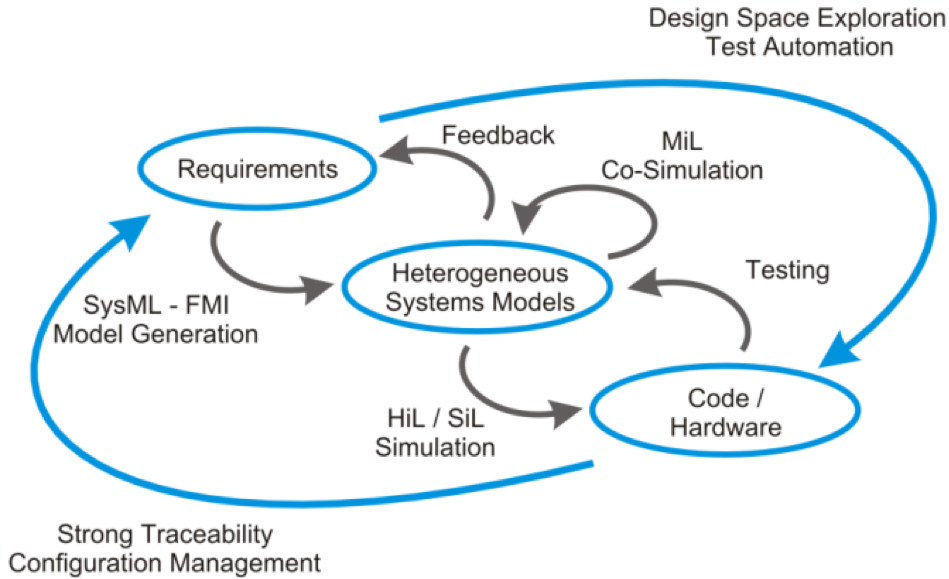
\includegraphics[width=\textwidth]{./figures/INTOoverview}
\caption{Connections in the INTO-CPS tool chain.}
\label{fig:intooverview}
\end{figure}

The goals of the INTO-CPS project have been to:
\begin{enumerate}
\item Build an open, well-founded tool chain for multidisciplinary model-based design of CPS that covers the full development life cycle of CPS.
\item Provide a sound semantic basis for the tool chain.
\item Provide practical methods in the form of guidelines and patterns that support the tool chain.
\item Demonstrate the effectiveness of the methods and tools in an industrial setting in a variety of application domains.
\item Form an INTO-CPS Association to ensure that results extend beyond the life of the project.
\end{enumerate}

\subsection{How INTO-CPS works}

The INTO-CPS project had a consortium consisting of 11 partners (four universities, seven companies) who contribute with complementary knowledge, baseline technologies and applications. The baseline technologies support systems modelling (Modelio), modelling and simulation of physical systems (OpenModelica, 20-sim), discrete-event modelling and simulation (Overture), Co-Simulation (Crescendo, TWT Co-Simulation engine) and test automation (RT-Tester). These baseline technologies enable both descriptions of Discrete Event (DE) models as well as Continuous-Time (CT) models. Any number of such constituent models may be combined in a hybrid setting using the INTO-CPS technology. Advancing over technologies commonly used today in industry, INTO-CPS provides an open tool chain that enables the following:

\begin{enumerate}
\item Providing a faster route to market for CPS products where control aspects depend upon the development of physical elements (e.g.\ mechanical parts) that typically take a long time to be developed.
\item Avoiding vendor lock-in by having an open tool chain that can be extended and used in different ways. Although it is well-founded it is based on pragmatic principles where a trade-off between accuracy and speed of analysis is enabled.
\item Including capabilities for exploring large design spaces efficiently so that ``optima'' solutions can be found given the parameters that are important for the user, both on the cyber and the physical side.
\item Limiting the necessity for large amounts of expensive physical tests in order to provide the necessary evidence for the dependability of the CPS.
\item Enabling traceability of all project artefacts produced by different tools using an open traceability standard.
\end{enumerate}

A Co-simulation Orchestration Engine (COE) called Maestro has been built on the baseline technologies and in accordance with requirements driven by the industry case studies outlined below \cite{Thule&17}. This engine combines previous experience from TWT's Co-Simulation engine and the Crescendo tool developed in the project Design Support and Tooling for Embedded Control Software (DESTECS) \cite{Broenink&10}. The goals for the COE include, among others, optimised scalability and performance, and data exchange between the different models facilitated by the Functional Mockup Interface (FMI) \cite{FMIStandard2.0}. Interfaces to further tools will be provided so that the requirements and the different artefacts will be fully exploited. An INTO-CPS Application acting as a common front-end to the INTO-CPS tool chain has been produced using web-based technologies (on top of Electron). This enables stakeholders without detailed knowledge on the different modelling technologies to experiment with alternative candidate designs and use systematic ways to either explore a large design space or systematically test heterogeneous models. The INTO-CPS Application, the COE and its most important connections are shown in Figure~\ref{fig:toolchain}. 
 
\begin{figure}[ht]
\centering
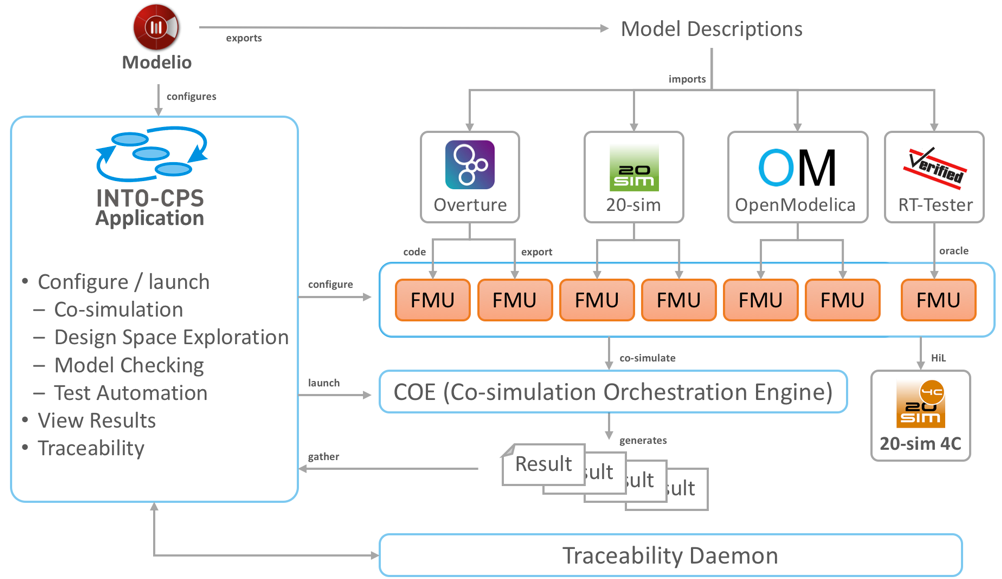
\includegraphics[width=\textwidth]{./figures/toolchain}
\caption{Overview of the INTO-CPS tool chain.}
\label{fig:toolchain}
\end{figure}

The COE connects multiple diverse models, each in the encapsulated form of a Functional Mock-up Unit (FMU) or running in its native modelling environment, to an overall system model. An algorithm for Design Space Exploration (DSE) enables sweeps through ranges of design parameters, performing co-simulations on each. System robustness can be evaluated by using Test Automation (TA) tools that can manipulate the simulation. Links to models can be kept in a database to allow for versioning and traceability even between artefacts produced by different tools. The INTO-CPS tool chain is described in more detail in Section~\ref{sec:toolchain}.
%The entire co-simulation is controlled from a user interface. The final year of the project has seen a significant investment in promoting the co-simulation capabilities, and \url{http://fmi-standard.org/tools/} has been set up as a core webpage for all tools supporting FMI-based co-simulations.

%During Year 3, the COE has been extended with capabilities both for distributed co-simulations and nested co-simulations. A graphical front-end for the entire tool chain called the INTO-CPS Application has been extended considerably. This has been developed further as a desktop application, using web technologies to enable a smoother transition to delivering this as an on-line service should this be desirable in the future . Building on the work of previous years, a 3D FMU support unit has been improved significantly, and has been used for multiple models, including those employed in the industrial case studies.

%Year 3 have seen advances in many other areas of the technology, including new features for Design Space Exploration (DSE), Test Automation (TA), Model Checking (MC), traceability and Code Generation (CG). All of these features have been integrated in the INTO-CPS Application. The final version of the DSE support has been augmented with a capability to deploy DSE on cloud services, making DSE a technology that can be used by businesses without large-scale compute resources of their own. Our SysML profile, designed to ease the high-level development of multi-models, has been extended with features to support disciplined approaches to DSE. The TA and MC capabilities already incorporated in the INTO-CPS Application have been improved during Year 3. Finally, the CG features are incorporated in the different baseline modelling, and simulation tools have been improved in terms of performance and integration. The full deployment of the CG features in a distributed and embedded setting turned out to require more resources than originally envisaged. Most importantly, the support for traceability between different CPS artefacts has been developed during Year 3, including extensions of all the baseline tools with Open Source Life Cycle (OSLC) support. It also turned out that more effort was needed for the full traceability support compared to what was originally envisaged.

\subsection{Industrial Case studies}
Inside the INTO-CPS project four industry-led case studies from different application domains have allowed us to evaluate the final INTO-CPS tool chain. These cases (and a couple of industrial cases conducted by external companies) are described further in~\autoref{sec:casestudies}. A brief overview of the industrial cases inside the INTO-CPS project and their main challenges are:

In the Railways case study led by the French company ClearSy, an innovative distributed interlocking solution has been developed, where signalling safety rules take both the logic and the physical conditions into account with a higher degree of independence than normally. The challenge was to find the right trade-off between the efficiency of an interlocking system (availability of routes, trains' delays and cost of interlocking system) and safety (collision avoidance, derailment prevention, availability and efficiency of the emergency system).

The Agriculture case study led by the Danish company Agrointelli concerns both an automated control system for an agricultural robot as well as an autonomously operating lawn mower. The robot, which provides more efficient removal of weeds in the field while operating safely but with minimal human interaction. In addition, the development of the autonomous control for the lawn mower was carried out. The challenge in both cases was to simulate the behaviour of physical components (such as mechanical loading on certain elements) together with controls of the automated system even before the physical mechanical components are available. These controls access local data (e.g. sensors) and external data (e.g.\ GPS). Model-based design allowed for accelerated time-to-market and virtual verification while reducing the need for multiple physical prototypes. 
%The Year 3 case study also demonstrated that reuse of ideas was possible in the sense that using the INTO-CPS technology development is faster compared to the traditional alternative.

In the Building Automation case study led by the Irish part of United Technology Research Centre (UTRC), CPSs for control of Heating, Ventilation and Air-conditioning (HVAC) have been developed. These CPSs need to be adaptable to components of various manufacturers and different building patterns and the corresponding requirements. The challenge here is also to manage the complexity of the overall system in a way so the co-simulations are sufficiently scalable. The various parts that influence an HVAC system have been modelled and simulated, e.g.\ the fan-coil unit that distributes air, the buildings and rooms as well as the controllers of the fan-coil units. 
%During Year 3 the team has been focusing on evaluating the scalability of the INTO-CPS co-orchestration engine to HVAC models of increased complexity. In the Year 3 use case, the chiller model has been introduced in order to challenge the efficiency and execution of co-simulations using INTO-CPS technology since we have experienced that even commercial tools often fail to deliver the required performance here. 
In addition, UTRC has run an extensive evaluation of all INTO-CPS features including DSE, test automation, Hardware-in-the-Loop (HiL) and 3D co-simulation.   

In the Automotive case study led by the German company TWT, a range optimisation assistant for electric vehicles is being developed. In order to maximise the range without compromising other qualities such as comfort or speed, a comprehensive assessment of the vehicle and its environment is necessary. To achieve this goal, all relevant parts of the system have been modelled, e.g.\ battery, drive train, topography, traffic, weather and cabin thermal control. These constituent models are created in native industrial tools, such as Matlab, and coupled using the INTO-CPS tool suite.

%In Year 3, the final INTO-CPS technologies have been used in all four case studies to get experience with these. 
In order to properly compare the INTO-CPS technology under development with existing modelling and simulation tools, some of the industrial case studies have, on purpose, developed some of their constituent models using such legacy tools (AI has used Gazebo, UTRC has used Dymola and TWT has used Matlab) in order to experiment with the FMUs exported from them in connection with the COE and the rest of the INTO-CPS tool chain. Generally speaking, the results have been quite positive. 
%All four industrial case studies have been extended in different ways (compared to Year 2) and as documented in D1.3a [INTO-CPS-D1.3] progress has been achieved in the assessment of the industrial needs for all four industrial case studies.

\subsection{The INTO-CPS foundations}

The development of tools and methods in INTO-CPS is based on a sound semantic description of co-simulation. Our tools use VDM-RT as the discrete-event language and Modelica as the continuous-time language. The framework for co-simulation is based on FMI. Both languages have been formalised and mechanised in this framework using Isabelle/UTP. We have a semantics of the relevant parts of SysML that can be used with FMI. These foundations allow for the formal checking of the validity of analysis and co-simulation results. There has also been a close integration with the industrial case studies (in particular, the railways and building applications) and supported the development of the INTO-CPS tool chain. It has been demonstrated how to use the foundational tools, with both theorem proving and model checking, to add value to the INTO-CPS tool chain. The foundations are described in more detail in~\autoref{sec:foundations}.

\subsection{The INTO-CPS methods and guidelines}

Lowering the barriers to multidisciplinary model-based engineering of CPSs demands methods that permit the deployment of tools in industry processes, embodied in guidelines that reflect experience gained using such methods. We present our modelling methods as guidelines for applying the INTO-CPS tool chain in real industry contexts, with a strong focus on supporting systematic DSE, our form of tradespace analysis, and on managing the traceability of design artefacts. All of the methods and guidelines materials have been made ready for subsequent use by the INTO-CPS Association.  

In order to ease practical deployment of INTO-CPS technology, a SysML profile has been developed to enable designers to move more readily from abstract system models to the structure of heterogeneous co-models. Thus, it has been extended with the ability to help engineers describe explicitly the parameters, objectives and ranking involved in the DSE process, and to allow sweeps to be made both over parameters and operating scenarios. We have developed a Traceability Information Model (TIM) that supports the needs of heterogeneous CPS engineering teams. In defining permissible relations between artefacts and activities, we have drawn on two sources: Open Services for Lifecycle Collaboration (OSLC)  and W3C PROV supported traceability links.

Our guidelines have been implemented in training materials and pilot studies which have been made publicly available and can readily be imported into the INTO-CPS Application, making it easy for newcomers to experiment with the INTO-CPS tools and methods. The pilots provide coverage of all INTO-CPS simulation technologies (VDM-RT, 20-sim and OpenModelica), have architectural models in SysML using the INTO-SysML profile, may be co-simulated with the INTO-CPS Application, can perform DSE, use code generation and have support for test automation. The methods and guidelines are described in more detail in~\autoref{sec:method}.
